\documentclass[nosymbols]{beamer}	% Is better for some Windows user.
%
\usepackage{pict2e}
\usepackage{tikz}
\def\UDM{ % untere Dreiecks-Matrix
\mbox{
\setlength{\unitlength}{9pt}
\begin{picture}(1,1)
\put(0,1){\line(1,0){1}}
\put(1,0){\line(0,1){1}}
\put(0,1){\line(1,-1){1}}
\end{picture}
}}
\title{Homogenization}
\author{Janna Puderbach}
% \input{docinfo}				% Edit here author informations.
% \input{header}
% \input{titlepage}
% \input{headingsandfooter}
\usepackage{algorithm2e}
\begin{document}
    \addtocounter{framenumber}{-1}	% Exclude page from pagecounter.
	\begin{frame}[plain]
		\titlepage
	\end{frame}
	%
	%\setcounter{framenumber}{0}
	\frame{
		\frametitle{Content}
		\tableofcontents
	}



	\section{Introduction}

\begin{frame}{Introduction} %Motivation
Given a composite material %Bild
\begin{figure}
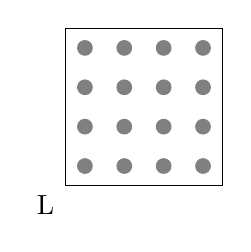
\begin{tikzpicture}
\draw (0.25,0.25) -- (0.25,2.25) -- (2.25,2.25) -- (2.25,0.25) -- (0.25,0.25);
\node (0,1.5){L};
  \foreach \x in {1,...,4}
    \foreach \y in {1,...,4}
        \fill[gray] (\x/2,\y/2) circle (1mm);
        
\end{tikzpicture}
\end{figure}
\textbf{microscopic scale}
\begin{itemize}
\item fine scale of inhomogeneous part
\item too expensive to solve with FEM
\end{itemize}
\textbf{macroscopic scale}
\begin{itemize}
\item Consider the material as homogeneous
\item easy to solve
\end{itemize}
\end{frame}

% %Example
\begin{frame}
Example
\begin{align*}
- \operatorname{div} (\sigma(x) \nabla u) &= g(x), \quad & x \in \Omega \\
u &= U , \quad & x \in \partial \Omega
\end{align*}

\begin{tikzpicture}
\draw  ;
\end{tikzpicture}
\end{frame}
%
\begin{frame}
\begin{align*}
\varepsilon = \frac{l}{L} \ll 1
\end{align*}
\end{frame}
\section{Homogenization problem}
%Homogenized problem
\begin{frame}
\begin{align*}
-\operatorname{div} (\sigma(\frac{x}{\varepsilon}) \nabla u_{\varepsilon}) &= g(x) , \quad & x \in \Omega\\
u_{\varepsilon} &= 0, \quad &x \in \partial \Omega
\end{align*}
\begin{align*}
u_{\varepsilon} &\rightharpoonup u_0 &\text{ weakly in } &H^1_0(\Omega)\\
\sigma_{\varepsilon}\nabla u_{\varepsilon} &\rightharpoonup \hat \sigma \nabla u_0 &\text{ weakly in } &L^2(\Omega)
\end{align*}
\end{frame}

\begin{frame}{Effective Conductivity Tensor}
\begin{align*}
\hat \sigma_{i,j} = \frac{1}{|\Pi|} \int_{\Pi} (\sigma(y)(\nabla \chi_i + \boldsymbol e_i)) \cdot (\nabla \chi_j + \boldsymbol e_j) \operatorname d y
\end{align*}
\end{frame}

\begin{frame}{Cell problem}
\begin{align}
- \operatorname{div} \left[ \sigma(y)[\nabla \chi_i + \boldsymbol e_i ]\right] = 0 , \quad y \in \Pi
\end{align}
\begin{figure}
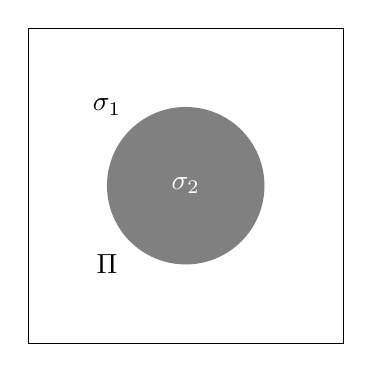
\begin{tikzpicture}
\draw  (0,0) -- (4,0) -- (4,4) -- (0,4) -- (0,0);
\draw[white] (1,3) circle (0.2cm) node[black]{$\sigma_1$};
\draw[white] (1,1) circle (0.2cm) node[black]{$\Pi$};
\fill[gray] (2,2) circle (1cm) node[white]{$\sigma_2$};
\end{tikzpicture}
\caption{Unit cell}
\end{figure}
\end{frame}
%
% %formal asymptotic expansion
\begin{frame}{Formal Asymptotic Expansion}
slow and fast variables independent
\begin{align}
u_{\varepsilon} (x) = u_0(x,\frac{x}{\varepsilon}) + \varepsilon u_1(x,\frac{x}{\varepsilon}) + \varepsilon^2 u_2(x,\frac{x}{\varepsilon}) + ...
\end{align}
\end{frame}
%
\section{Two-Scale Convergence}
%Two-scale convergence
\begin{frame}{Two-Scale Convergence}
% \textbf{Strong Convergence}

\textbf{Weak Convergence}


\textbf{Two-Scale convergence}
\begin{align*}
\lim_{\varepsilon \to 0} \int_
{\Omega} u_\varepsilon (x) \Psi(x,\frac{x}{\varepsilon}) \operatorname d x = \int_{\Omega} \int_\Pi u_0(x,y) \Psi(x,y)\operatorname d y \operatorname d x
\end{align*}
\end{frame}
%\begin{frame}{Quellen}

%\end{frame}

% \begin{frame}
% \begin{center}
%     \begin{huge}
%     Vielen Dank für Ihre Aufmerksamkeit!\\[1,5cm]
%     Fragen?
%     \end{huge}
% \end{center}
%
% \end{frame}

\end{document}
